La compilation sous windows est bien plus simple. Pour ce faire vous pouvez utiliser Visual Studio Code ( VS Code) par exemple. \\

Il vous faut ouvrir VS Code puis faire Fichier => Ouvrir Dossier => puis sélectionner le dossier racine du projet comme ci-dessous => puis faire \textbf{Sélectionner un dossier}.
\begin{figure}[h]
    \centering
    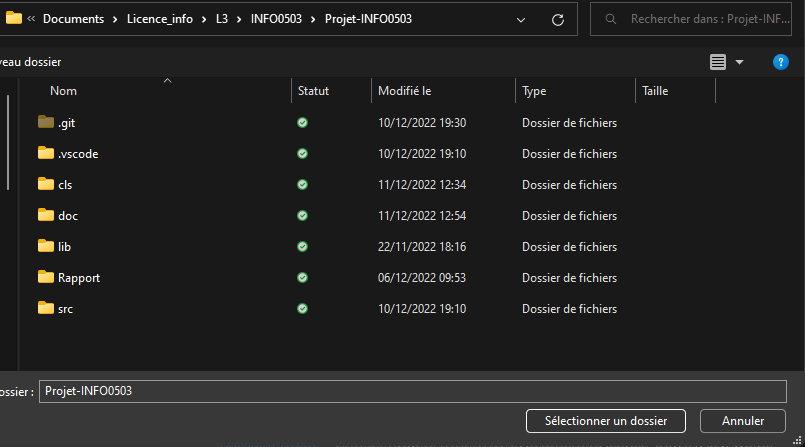
\includegraphics[width= 150mm, height=75mm]{images/FichierASelectionner.png}
    \caption{Dossier à selctionner}
    \label{img:mesh6}
\end{figure}


Une fois le projet ouvert vous pourrez voir sur la gauche de l'interface de VS Code, l'ensemble des dossiers et sous-dossiers contenant les fichiers ".java" du projet, soit l'arborescence du projet.

Une fois que VS Code a reconnu le projet JAVA. Rendez-vous dans le fichier "Lanceur.java", puis dirigez vous à la ligne 28, vous y trouverez un bouton \textbf{Run | Debug} comme sur la figrue suivante.
\begin{figure}[h]
    \centering
    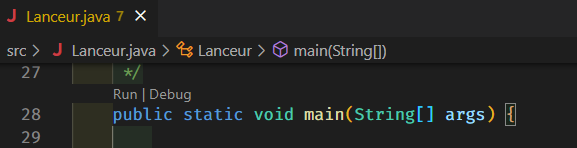
\includegraphics[width= 80mm, height=30mm]{images/BoutonRunDebug.png}
    \caption{Bouton Run | Rebug}
    \label{img:mesh7}
\end{figure}

Il vous suffit de presser le bouton \textbf{Run}, à ce moment là le terminal VS Code se lance mais une erreur apparait comme sur la figure suivante.

\begin{figure}[h]
    \centering
    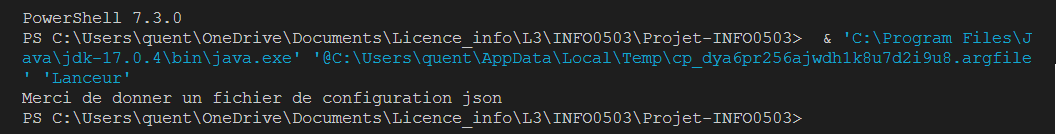
\includegraphics[width= 139mm, height=17mm]{images/ErreurVSCODE.png}
    \caption{Erreur de compilation VSCode}
    \label{img:mesh8}
\end{figure}

Pour résoudre ce problème, il vous suffit de vous rendre dans votre dossier ".vscode" puis dans le fichier 'launch.json" et d'ajouter dans "projectName" la ligne suivante : "args":"config.json" comme sur la figure suivante.

\begin{figure}[h]
    \centering
    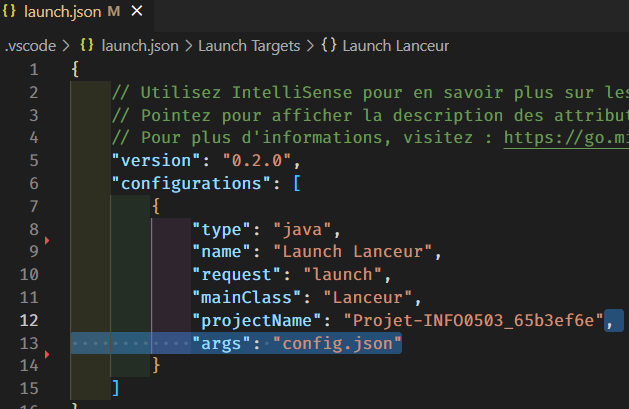
\includegraphics[width= 83mm, height=54mm]{images/lauchjson.png}
    \caption{Ajout de "args"}
    \label{img:mesh9}
\end{figure}

Une fois cette ligne ajoutée, vous pouvez relancer avec le bouton \textbf{Run} et vos serveurs seront opérationnels.
\begin{figure}[h]
    \centering
    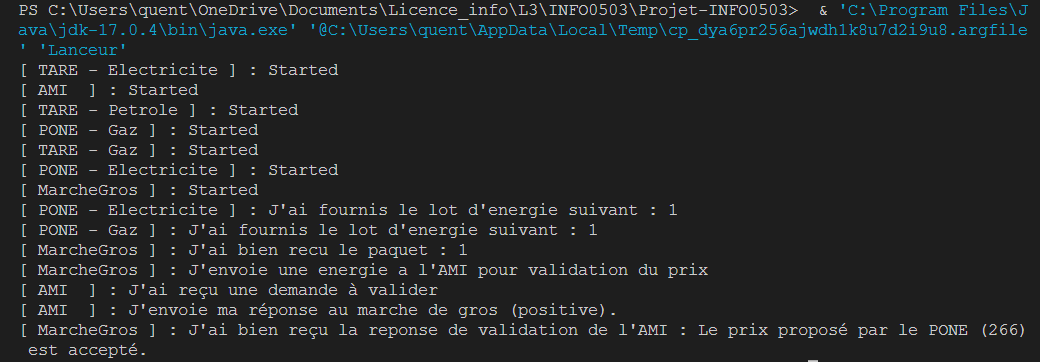
\includegraphics[width= 137mm, height=43mm]{images/VScodeProject.png}
    \caption{Lancement du serveur}
    \label{img:mesh10}
\end{figure}

\newpage